\section{Operationen}
Nachdem ein Half-Edge Mesh prozedural erstellt wurde oder ein Unity Mesh umgewandelt wurde, k\"onnen auf ein Half-Edge Mesh einige Standardoperationen angewendet werden. Folgende Operationen werden im folgenden Kapitel erkl\"art und die Implementierung beschrieben:
\begin{itemize}
	\item das Teilen einer HalfEdge (Split HalfEdge),
	\item das Kollabieren einer Kante (Edge Collapse),
	\item das Aufteilen einer Face (Subdivision) und
	\item eine einfache 2D-Zerst\"orungssimulation (Simulate Breaking).
\end{itemize}

\subsection{Split Half-Edge}
Ziel der \textit{SplitHalfEdge}-Methode ist es, eine HalfEdge so zu teilen, dass das Ergebnis der Operation ein konformes Half-Edge Mesh ist, also dass jede Face immer noch aus drei Half-Edges besteht und dass jede Half-Edge maximal einen Partner besitzt. Um das Teilen durchzuf\"uhren, m\"ussen folgende Schritte durchgef\"uhrt werde, die in der Abbildung \ref{fig:splithalfedge} schematisch dargestellt sind:
\begin{enumerate}
	\item Bestimme die zu splittende HalfEdge.
	\item Erzeuge einen neuen Punkt, dort wo sich die HalfEdge aufteilt.
	\item Erzeuge drei neue HalfEdges und eine neue Face:
	\begin{itemize}
		\item Eine HalfEdge zum neuen Punkt, vom Ursprung der gesplitteten HalfEdge
		\item Eine HalfEdge als Nachfolger der ersten HalfEdge, mit dem neuen Punkt als Ursprung 
		\item Eine HalfEdge als Vorg\"anger der gesplitteten HalfEdge
	\end{itemize}
	\item Setze die Referenzen der HalfEdges neus
	\item F\"uhre Schritte 1-4 f\"ur die der gesplitteten HalfEdge gegen\"uberliegende HalfEdge ebenfalls aus
	\item Setze die Paare neu
\end{enumerate}

\begin{figure}[H]
	\centering
	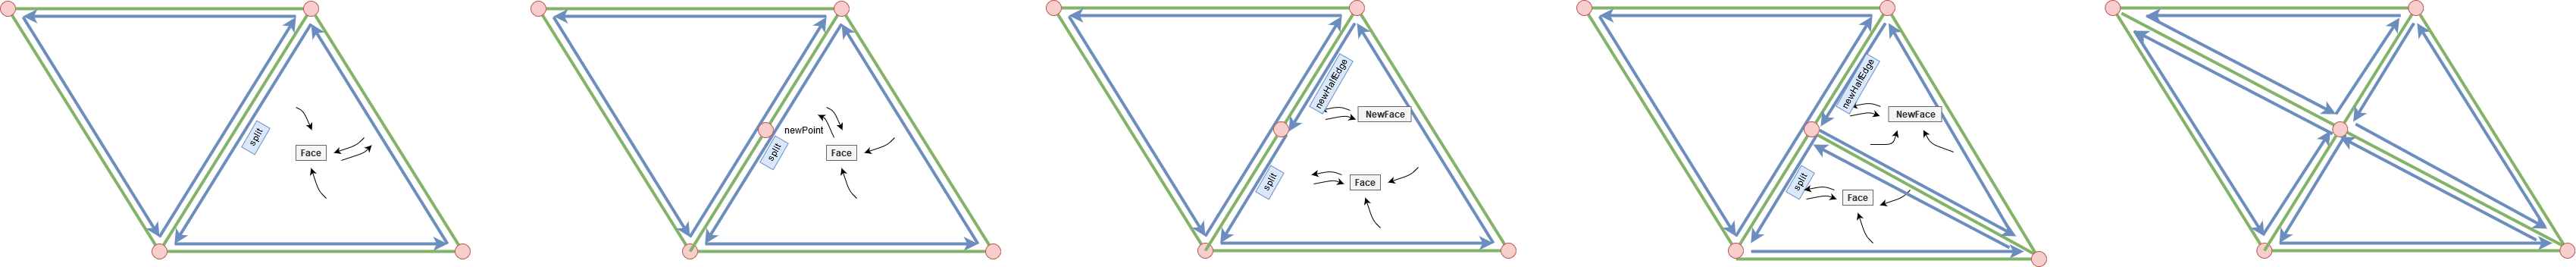
\includegraphics[width=1\linewidth]{Images/splitHalfEdge}
	\caption{Schematische Darstellung eines Edgesplits. In Bild 1 ist die Ausgangssituation dargestellt, Bild 2 zeigt Schritt 2, die Bilder 3 und 4 zeigen die Schritte 3 und 4 und Bild 5 zeigt das Ergebnis, nach den Schritten 5 und 6.}
	\label{fig:splithalfedge}
\end{figure}


Der beschriebene Algorithmus ist im Folgenden implementiert:
\begin{lstlisting}
private bool _lock = false;
private HalfEdge _newHalfEdge, _split;

public void SplitHalfEdge(HalfEdge split, Vector3 splitPoint)
{
	// --- Schritt 1:
	split.Face.HalfEdge = split; // --- Set Reference of 
	// --- Face to split to know where the new face goes
	_split = split;

	// --- Schritt 2:
	Vertex newPoint = _mesh.Vertices.CreateVertex(splitPoint);

	// --- Schritt 3:
	HalfEdge newHalfEdge = _mesh.HalfEdges
	.CreateHalfEdge(split.OutgoingPoint, null, split);
	_newHalfEdge = newHalfEdge;
	Face newFace = _mesh.Faces.CreateFace(newHalfEdge);
	split.OutgoingPoint = newPoint;

	HalfEdge newHalfEdgeToSplit = _mesh.HalfEdges
	.CreateHalfEdge(split.Next.EndPoint, split.Face, split);
	HalfEdge newHalfEdgeFromNewHalfEdge = _mesh.HalfEdges
	.CreateHalfEdge(newPoint, newFace, split.Next.Next);
	_mesh.HalfEdges
	.CreatePair(newHalfEdgeToSplit, newHalfEdgeFromNewHalfEdge);

	// --- Schritt 4:
	newHalfEdge.Next = newHalfEdgeFromNewHalfEdge;
	newHalfEdgeFromNewHalfEdge.Next.Next = newHalfEdge;
	split.Next.Next = newHalfEdgeToSplit;

	// --- Aktualisiere das Unity Mesh
	_mesh.AddMeshVertex(newPoint.Point);
	
	_mesh.SetMeshTriangles(split.Face.Index,
	_mesh.Faces.GetFaceCirculator(split.Face)
	.Select(p => p.OutgoingPoint.Index)
	.ToList(), true);
	 
	_mesh.SetMeshTriangles(newFace.Index,
	_mesh.Faces.GetFaceCirculator(newFace)
	.Select(p => p.OutgoingPoint.Index)
	.ToList(), true);
	
	if (!_lock) // --- Blockiere nach dem ersten Aufruf,
				// --- um eine Endlosschleife zu vermeiden
	{
		// --- Schritt 5:
		if (split.Opposing != null) 
		{
			_lock = true;
			SplitHalfEdge(split.Opposing, splitPoint);
			// --- Schritt 6:
			_mesh.HalfEdges.CreatePair(_split, newHalfEdge);
			_mesh.HalfEdges.CreatePair(split, _newHalfEdge);
			_lock = false;
		}
	_mesh.CommitMeshTriangles();
	}
}
\end{lstlisting}
In wird die \textit{SplitHalfEdge}-Methode auf das erste Mesh in Abbildung \ref{fig:meshmash} angewendet, so ist das Mesh im zweite Bild das Ergebnis, wenn die Diagonale gesplittet wird und im Dritten, wenn die linke Kante unterhalb der Mitte geteilt wird. Das letzte Bild zeigt, dass der Teilungspunkt nicht zwingend auf der Kante liegen muss, da sich die Kanten entsprechend anpassen.
\begin{figure}[H]
	\centering
	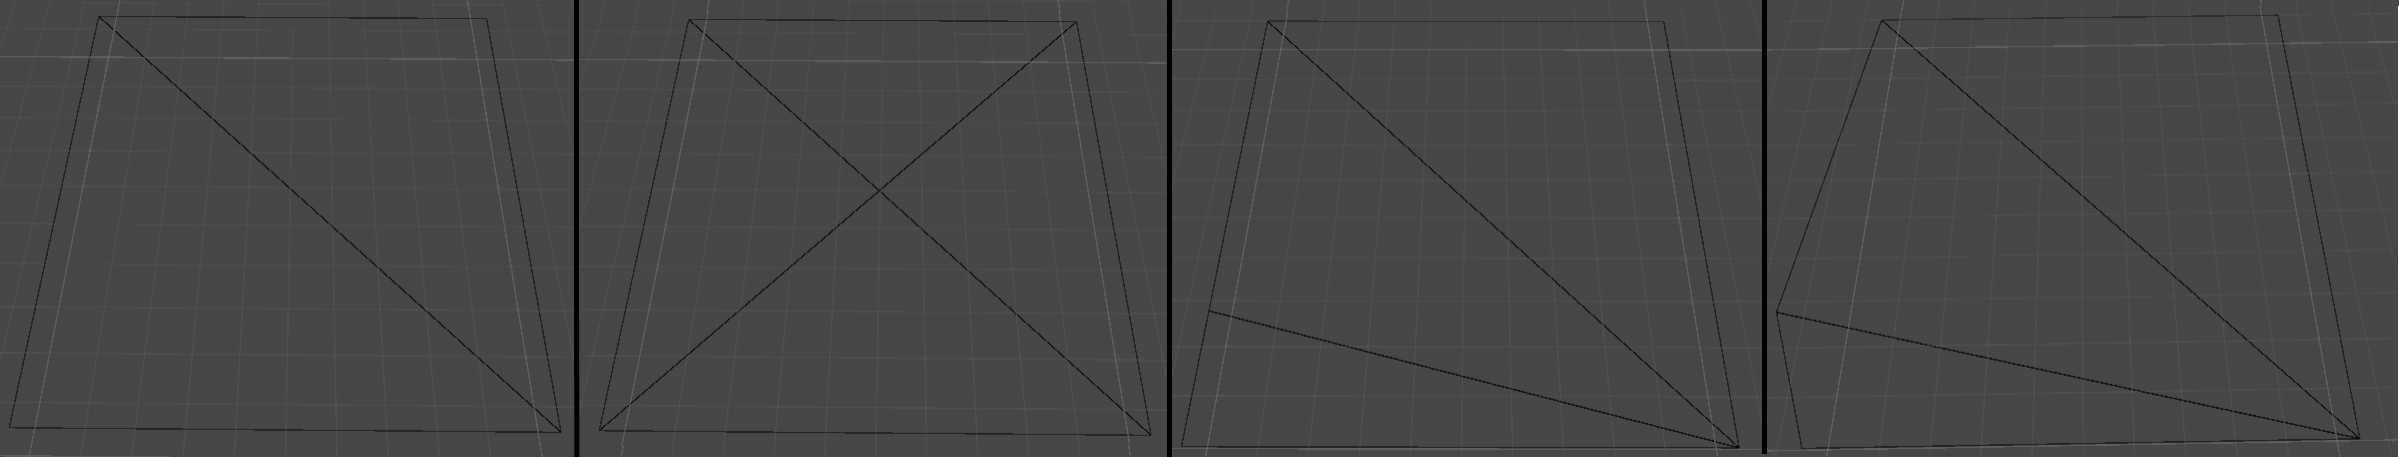
\includegraphics[width=1 \linewidth]{Images/meshmash}
	\caption{Bild 1 ist das Ausgangsmesh, welches in Bild 2 in der Mitte der Diagonale gesplittet wurde, in Bild 3 ein viertel auf dem Weg nach oben, auf der linken Seite und im 4. Bild eine Einheit links von der Kante}
	\label{fig:meshmash}
\end{figure}

Der beschriebene Algorithmus besitzt eine konstante Laufzeit, da alle \"Anderungen lokal an den betroffenen HalfEdges vorgenommen werden k\"onnen und die einzigen ,,komplexen'' Operationen auf der \textit{GetFaceCirculator}-Methode basieren, die immer die drei anliegenden HalfEdges einer Face zur\"uckgibt. Wird im Gegensatz dazu die selbe Operation nur mithilfe vom UnityMesh versucht, so m\"usste mittels Brute-Force zuerst jeder Index der Eckpunkte der gesuchten Kante ermittelt werden, da diese nicht explizit dargestellt wird, um anschlie{\ss}end in den Indices die Dreiecke zu finden, die diese Eckpunkte verwenden, damit diese durch die neu bestimmten Dreiecke ersetzt werden k\"onnen. Daraus resultiert einen Laufzeit, in Abh\"angigkeit von der Anzahl der Vertices im Netz, wodurch es zu Performanceproblemen bei gro{\ss}en Netzen kommen kann.

\subsection{Edge Collapse}
Der Edge-Collapse ist eine Operation, die dazu dient, die Komplexit\"at eines Models zu reduzieren. Dabei werden zwei Punkte zusammengef\"uhrt, indem eine Kante zusammenf\"allt, wodurch bei einer Operation zwei Dreiecksfl\"achen entfernt werden, ohne die gesamte Struktur zu ver\"andern \cite{Castello07}. In diesem Ansatz kann bestimmt werden, zu welchem Punkt die Kante zusammenf\"allt, je nachdem, welche der beiden HalfEdges als Ursprung gew\"ahlt wird, da daf\"ur der Endpunkt der HalfEdge verwendet wird. 
Um einen Edge-Collapse durchzuf\"uhren, m\"ussen die Schritte aus Abbildung \ref{fig:edgecollapse} befolgt werden:
\begin{enumerate}
	\item Bestimme die an der HalfEdge anliegenden Vertices, HalfEdges und Faces.
	\item Setze die Referenzen der Nachbarschaftsbeziehung neu, die Nachbarn der HalfEdges die an der selben HalfEdge liegen und nicht teil der kollabierenden Kante sind werden Nachbarn.
	\item Entferne die betroffene Faces und HalfEdges.
	\item Setze alle Referenzen von einem Vertex auf den andern, entferne den Unbenutzten.
\end{enumerate}
\begin{figure}[H]
	\centering
	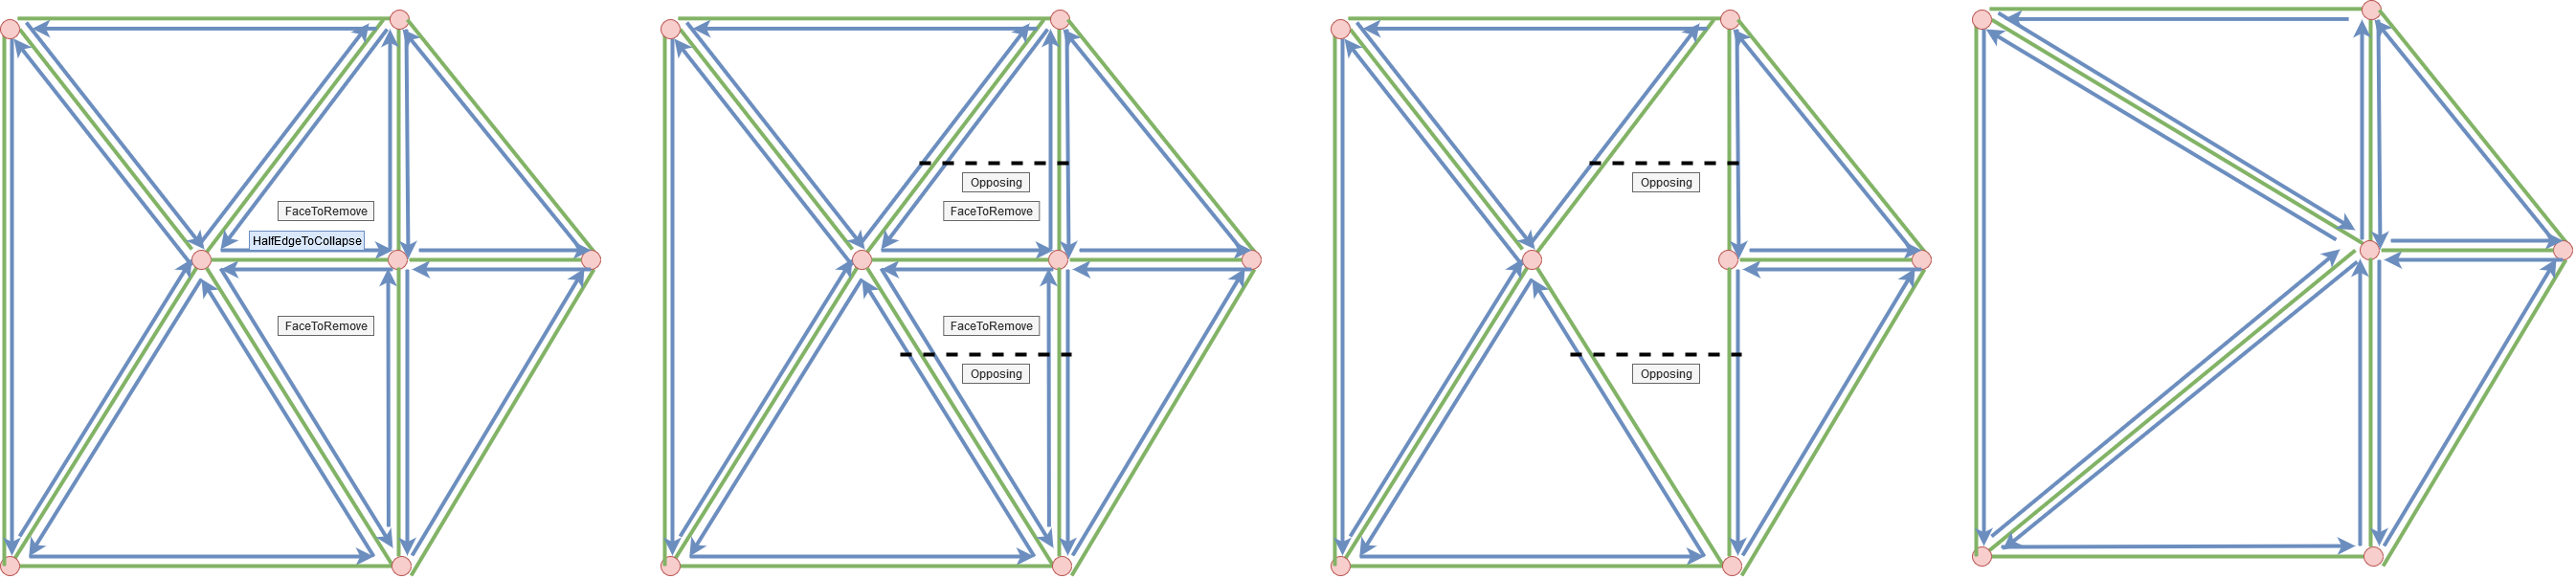
\includegraphics[width=1\linewidth]{Images/EdgeCollapse}
	\caption{Schematische Darstellung des Edge-Collapses. Bild 1 zeigt die Ausgangssituation, Bild 2 stellt die neuen Nachbarschaftsreferenzen dar, in Bild 3 wurden die Faces entfernt und in Bild 4 ist das Ergebnis zu sehen.}
	\label{fig:edgecollapse}
\end{figure}
Die Implementierung des beschriebenen Algorithmus sieht folgenderma{\ss}en aus:
\begin{lstlisting}
public void EdgeCollapse(HalfEdge halfEdge)
{
	// --- the point the halfEdge is collapsing to
	Vertex collapsingPoint = halfEdge.EndPoint;
	Vertex pointToRemove = halfEdge.OutgoingPoint;

	// --- determine the halfEdges to remove
	// --- those are the HalfEdges around the halfEdge Face 
	// --- and it's pairs face
	HalfEdge pair = halfEdge.Opposing;

	List<HalfEdeg> halfEdgesToRemove =
	_mesh.Faces.GetFaceCirculator(halfEdge.Face);
	halfEdgesToRemove
	.AddRange(_mesh.Faces.GetFaceCirculator(pair.Face));

	// --- set the neighbours right
	foreach(HalfEdge he in halfEdgesToRemove)
	{
		if (he.Index == halfEdge.Index 
		|| he.Index == pair.Index 
		|| he.Next.Index == halfEdge.Index 
		|| he.Next.Index == pair.Index
		|| he.Opposing == null 
		|| he.Next.Opposing == null)
			continue;

		_mesh.HalfEdges.CreatePair(he.Opposing, he.Next.Opposing);
	}

	_mesh.Faces.RemoveFace(halfEdge.Face);
	_mesh.Faces.RemoveFace(pair.Face);

	foreach (HalfEdge he 
	in _mesh.Vertices.GetVertexCirculator(pointToRemove))
	{
		if(he.OutgoingPoint.Index == pointToRemove.Index)
		{
			he.OutgoingPoint = collapsingPoint;
		}
	}

	_mesh.Vertices.RemoveVertex(pointToRemove);
	_mesh.GenerateUnityMesh();
}
\end{lstlisting}
Die Methode \textit{RemoveFace} ist eine Methode aus der \textit{FaceList} und regelt auch das L\"oschen von allen weiteren Referenzen:
\begin{lstlisting}
public void RemoveFace(Face f)
{
	List<HalfEdge> halfEdges = GetFaceCirculator(f);
	foreach (var halfEdge in halfEdges)
	{
		if (halfEdge.Opposing != null)
		halfEdge.Opposing.Opposing = null;

		if(_mesh.Vertices.GetVertexCirculator(halfEdge.OutgoingPoint)
		.Count <= 0)
		{
			_mesh.Vertices.RemoveVertex(halfEdge.OutgoingPoint);
		}
	}
	_mesh.HalfEdges.RemoveAll(p => halfEdges.Contains(p));

	_faces.Remove(f);
}
\end{lstlisting}


\subsection{Subdivision}
Im Gegensatz zum Edge-Collapse kann es beim Arbeiten mit 3D-Modellen auch n\"otig sein, eine Face in mehrere kleinere Faces zu unterteilen, um den Detailgrad des Modells zu erh\"ohen oder Zerst\"orung realistischer zu modellieren. Um dies zu erreichen, bietet die \textit{FaceSplittingBehaviour}-Klasse die \textit{SplitFace}-Methode, die eine gegebene Face an einem gegebenen Punkt in drei kleinere Faces Aufteilt. Um dies zu erreichen muss:
\begin{enumerate}
	\item Der neue Punkt auf der Face erzeugt werden.
	\item F\"ur jede HalfEdge der Face:
	\begin{itemize}
		\item Eine HalfEdge vom Endpunkt der HalfEdge zum neuen Punkt erzeugt werden.
		\item Eine HalfEdge vom neuen Punkt zum Startpunkt der HalfEdge erzeugt werden.
		\item Eine Face (wenn n\"otig) erzeugt werden.
		\item Die ,,Next''-Referenz der HalfEdge auf die HalfEdge zum neuen Punkt gesetzt werden.
	\end{itemize}
	\item F\"ur jede neue HalfEdge der Partner gesetzt werden.
\end{enumerate}
\begin{figure}[H]
	\centering
	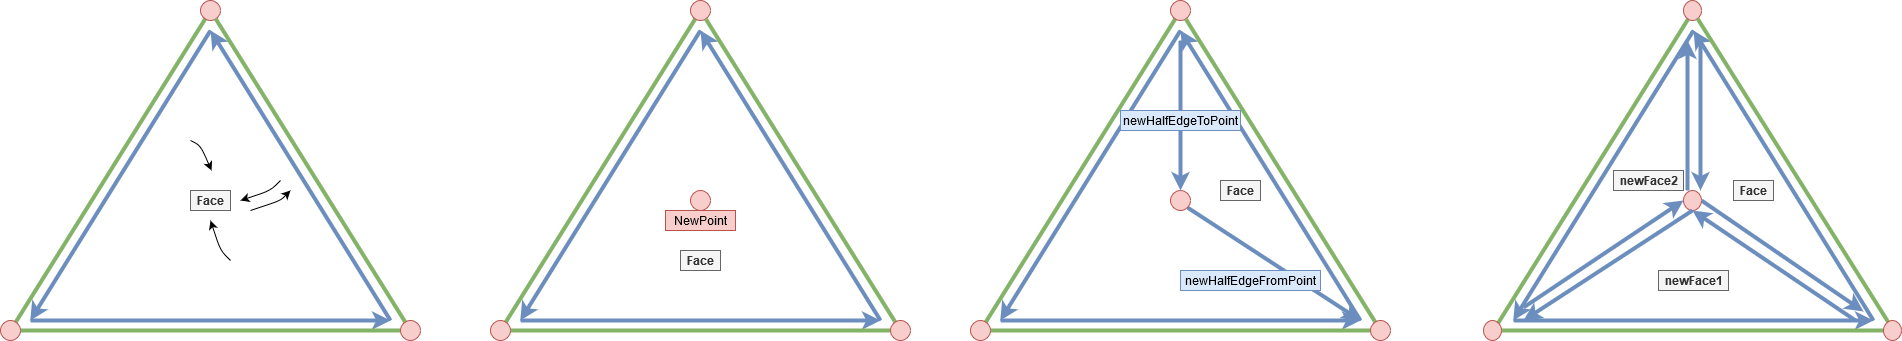
\includegraphics[width=1\linewidth]{Images/splitFace}
	\caption{Schematische Darstellung des SplitFace Algorithmus. Bild 1 zeigt die Ausgangsposition, Bild 2 zeigt Schritt 2, Bild drei einen Teilschritt von Schritt 3 und Bild 4 zeigt das Ergebnis}
	\label{fig:splitface}
\end{figure}

In C\# ergibt sich daraus der folgende Quellcode, welcher durch den \"Ubergabeparameter \textit{isTransaction} f\"ur den Gebrauch im gesamten Mesh optimiert ist.
\begin{lstlisting}
public void SplitFace(Face face, Vector3 pointToSplit, bool isTransaction = false)
{
	// --- Schritt 1:
	Vertex center = _mesh.Vertices.CreateVertex(pointToSplit);
	_mesh.AddMeshVertex(center.Point);

	// --- Schritt 2:
	List<HalfEdge> halfEdges = _mesh.Faces.GetFaceCirculator(face);
	List<HalfEdge> newHalfEdges = new List<HalfEdge>(); 
	// --- Keeping a reference to all new HalfEdges to pair them later

	// --- Schritt 3:
	for (int i = 0; i < halfEdges.Count; i++)
	{
		HalfEdge halfEdge = halfEdges[i];
		Face newFace = face;
		if (i == 0)        // --- reuse old face
		{
			newFace.HalfEdge = halfEdge;
		}
		else
		{
			newFace = _mesh.Faces.CreateFace(halfEdge);
		}

		HalfEdge newHalfEdgeFromCenter = _mesh.HalfEdges.CreateHalfEdge(center, newFace, halfEdge);
		HalfEdge newHalfEdgeToCenter = _mesh.HalfEdges.CreateHalfEdge(halfEdge.EndPoint, newFace, newHalfEdgeFromCenter);
		halfEdge.Next = newHalfEdgeToCenter;

		_mesh.SetMeshTriangles(newFace.Index, _mesh.Faces.GetFaceCirculator(newFace).Select(p => p.OutgoingPoint.Index).ToList(), true);
		newHalfEdges.AddRange(new List<HalfEdge> { newHalfEdgeFromCenter, newHalfEdgeToCenter, halfEdge });
	}
	
	// --- Schritt 4:
	_mesh.HalfEdges.CreatePair(newHalfEdges[0], newHalfEdges[4]);
	_mesh.HalfEdges.CreatePair(newHalfEdges[3], newHalfEdges[7]);
	_mesh.HalfEdges.CreatePair(newHalfEdges[6], newHalfEdges[1]);

	// --- Optimisation for SplitAllFaces
	if(isTransaction)
		_mesh.CommitMeshTriangles();
}
\end{lstlisting}

